\documentclass[UTF8]{article}
\usepackage{graphicx}
\usepackage{ctex}
\usepackage{amsmath}
\usepackage{amsfonts}
\usepackage{amssymb}
\usepackage{enumerate}
\usepackage{color}
\usepackage{setspace}
\usepackage{pythonhighlight}
\usepackage{bm}

\usepackage
[a4paper,
text={146.4true mm,239.2 true mm},
top= 26.2true mm,
left=31.8 true mm,
head=6true mm,
headsep=6.5true mm,
foot=16.5true mm]
{geometry} % 设置文本的边距
\input{../setup/format}

\begin{document}
\title{Homework 2 of Stochastic Processes}
\author{姓名:林奇峰\qquad 学号:19110977}
\maketitle

\section{Let $S_n=X_1+\cdots+X_N$ where $X_1,\dots,X_n$ are i.i.d binary rv.s with PMF $p_x(0) = \frac{3}{4}$ and $p_x(1)=\frac{1}{4}$.}
\begin{enumerate}
    \item Plot the CDF of $Yn=\frac{S_n-n\overline{X}}{n}$ for $n=4$, 20 and 50.
    \item Plot the CDF of $Z_n=\frac{S_n-n\overline{X}}{\sqrt{n}}$ for $n=4$, 20 and 50.
\end{enumerate}

\textbf{Solutions:}

\begin{enumerate}
    \item The figure of CDF of $Y_n=\frac{Sn-n\overline{X}}{n}$ is showed as following:
    \begin{figure}[h]
            \centering
            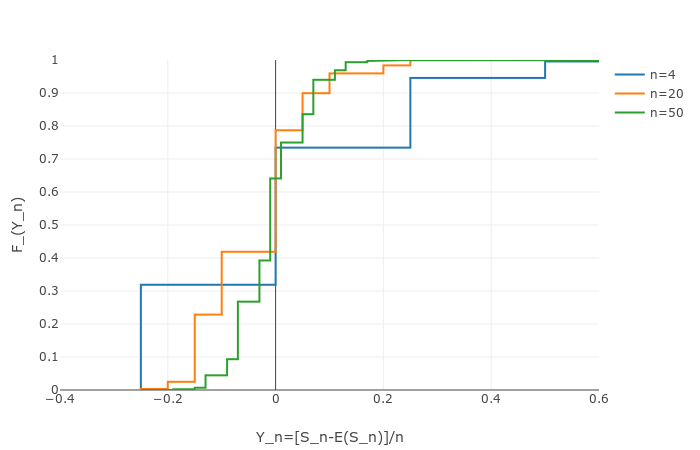
\includegraphics[width=5.0in]{wlln.png}
            \caption{CDF of $Y_n=\frac{Sn-n\overline{X}}{n}$}
            \label{fig:wlln}
        \end{figure}
    \item The figure of CDF of $Z_n=\frac{Sn-n\overline{X}}{\sqrt{n}}$ is showed as following:
    \begin{figure}[h]
            \centering
            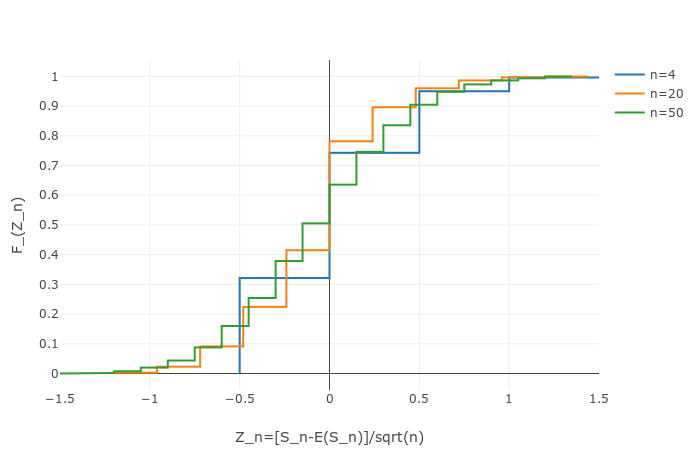
\includegraphics[width=5.0in]{clt.png}
            \caption{CDF of $Z_n=\frac{Sn-n\overline{X}}{\sqrt{n}}$}
            \label{fig:clt}       
        \end{figure}
\end{enumerate}

\newpage
\section{掷一个骰子}
\begin{enumerate}[a)]
    \item 写出样本空间$S$
    \item $\mathcal{F}_0=\{S,\emptyset,A\}$是一个事件类吗?其中$A=\{1,3,5\}$
    \item $\mathcal{F}_1=\{S,\emptyset, A, A^c\}$是一个事件类吗?$\mathcal{F}=2^S$呢?
    \item 定义$X=$骰子面上的点数
        \begin{enumerate}[i.]
            \item 若我们考察的概率模型是以$\mathcal{F}_1$为事件类,$X$是随机变量吗?
            \item 若我们考察的概率模型是以$\mathcal{F}$为事件类,$X$是随机变量吗?
        \end{enumerate}
    \item 定义$Y=X\text{mod}2$,讨论d)所讨论的问题。
    \item 思考题:随机变量的定义与概率$P(\cdot)$有关吗?
\end{enumerate}

\textbf{答:}

事件的公理定义如下:

Given a sample space $\Omega$, the class of subsets of $\Omega$ that consititue the set of events satisfies the following axioms:
\begin{enumerate}
    \item $\Omega$ is an events
    \item For every sequence of events $A_1,A_2,\dots,$ the union $\cup^\infty_{n=1}A_n$ is an event.
    \item For every event $A$, the complement $A^c$ is an event.
\end{enumerate}
\begin{enumerate}[a)]
    \item $S=\{1, 2, 3, 4, 5, 6\}$
    \item $\mathcal{F}_0=\{S,\emptyset,A\}$不是一个事件类。因为它违反了事件公理中的第三条,即$A^c$不在事件类中,构不成事件。
    \item   \begin{enumerate}[I.]
                \item $\mathcal{F}_1=\{S,\emptyset, A, A^c\}$是一个事件类。因为它满足所有的事件公理。
                \begin{enumerate}[i.]
                    \item 首先,样本空间$S$在事件类中,满足第一条事件公理。
                    \item 其次,对任意一个事件序列$E_1,E_2\dots$,$\cup^\infty_{n=1}E_n$也是一个事件,满足第二条事件公理。
                        \begin{enumerate}[(1)]
                            \item $\forall E_n=\emptyset, \cup^\infty_{n=1}E_n=\emptyset\in\mathcal{F}_1$。
                            \item $\exists E_n=S, \cup^\infty_{n=1}E_n=S\in\mathcal{F}_1$。
                            \item $\forall E_n=A, \cup^\infty_{n=1}E_n=A\in\mathcal{F}_1$。
                            \item $\forall E_n=A^c, \cup^\infty_{n=1}E_n=A^c\in\mathcal{F}_1$。
                            \item $\exists E_i=A, E_j=A^c\text{且}i\neq j, \cup^\infty_{n=1}E_n=S\in\mathcal{F}_1$。
                            \item $令B=\{m|A_m=\emptyset\},\text{则}\cup^\infty_{n=1}A_n=(\cup A_i)\cup(\cup A_j)=\cup A_j\text{其中}i\in B, j\notin B$。$\cup A_j$是上面(2)-(5)中的其中一种情况,因此$\cup^\infty_{n=1}E_n\in\mathcal{F}_1$。
                        \end{enumerate}
                        综上,$\cup^\infty_{n=1}E_n$是一个事件。
                    \item 对于任意一个事件$E$,其补集$E^c$也是一个事件,满足第三条事件公理
                        \begin{enumerate}[(1)]
                            \item 当$E=\emptyset$时,$E^c=S\in\mathcal{F}_1$。
                            \item 当$E=S$时,$E^c=\emptyset\in\mathcal{F}_1$。
                            \item 当$E=A$时,$E^c=A^c\in\mathcal{F}_1$。
                            \item 当$E=A^c$时,$E^c=A\in\mathcal{F}_1$。
                        \end{enumerate}
                \end{enumerate}
                综上,$\mathcal{F}_1$满足所有的事件公理。因此,$\mathcal{F}_1$是一个事件类。
                \item 当$\mathcal{F}=2^S$时,$\mathcal{F}$是一个事件类。
                    \begin{enumerate}
                        \item 首先,$S\in\mathcal{F}$,满足第一条事件公理。
                        \item 其次,对于任意一个事件序列$E_1,E_2\dots,\cup^\infty_{n=1}E_n$也是一个事件,满足第二条事件公理。因为$\mathcal{F}$是$S$的幂集,即$S$的所有子集都在$\mathcal{F}$中。
                        \item 对于任意一个事件$E$,其补集都在$\mathcal{F}$中,因此满足第三条事件公理。
                    \end{enumerate}
                    综上,$\mathcal{F}=2^S$是一个事件类。
            \end{enumerate}  
        \item 
            \begin{enumerate}[i.]
                \item  当考察的概率模型是以$\mathcal{F}_1$为事件类时,$X$不是一个随机变量。因为它不满足随机变量的一个性质:$\{\omega\in\Omega:X(\omega)\leq x\}$ is an event for each $x\in\mathbb{R}$。如$\{\omega\in\Omega:X(\omega)\leq2\}=\{1,2\}\notin\mathcal{F}_1$。
                \item 当考察的概率模型是以$\mathcal{F}$为事件类时,$X$是随机变量。首先,因为$\mathcal{F}$是$S$的所有子集的集合,则$\forall x\in\mathbb{R}$, $C=\{\omega\in\Omega:X(\omega)\leq x\}$都在$\mathcal{F}$中,即为一个事件。其次,$\forall x_1\in\mathbb{R},\dots,x_n\in\mathbb{R}$, $D=\{\omega:X_1(\omega)\leq x_1,\dots,X_n(\omega)\}$也都在$\mathcal{F}$中,即为一个事件。因此,$X$是随机变量。
            \end{enumerate}
        \item \begin{enumerate}[i.]
                    \item 当$Y=X\text{mod}2$且以$\mathcal{F}_1$为事件类时,$Y$是一个随机变量。根据定义,$Y$的取值为0或1。
                        \begin{enumerate}[(1)]
                            \item 当$y\in\mathbb{R}\text{且}y<0$时,$\{\omega:Y(\omega)\leq y\}=\emptyset\in\mathcal{F}_1$。
                            \item 当$y\in\mathbb{R}\text{且}0\leq y<1$时,$\{\omega:Y(\omega)\leq y\}=A^c\in\mathcal{F}_1$。
                            \item 当$y\in\mathbb{R}\text{且}1\leq y$时,$\{\omega:Y(\omega)\leq y\}=S\in\mathcal{F}_1$。
                            \item 从上面的讨论中我们已经可以知道,对于任意一个映射$Y$,它都满足以下性质:
                            
                            $\forall y\in\mathbb{R}, \{\omega:Y(\omega)<y\}$是一个事件。 
                            
                           则,$\forall y_1\in\mathbb{R},\dots,y_n\in\mathbb{R}$,令$D=\{\omega:Y_1(\omega)<y_1,\dots,Y_n(\omega)<y_n,\}=\cap^n_{i=1}D_i$,其中$D_i=\{\omega:Y_i(\omega)<y_1\}$。根据上述楞知$D_i\in\mathcal{F}_1$为一个事件,且根据事件公理$D_i^c\in\mathcal{F}_1$也是一个事件,所以根据事件公理,$\cap^n_{i=1}D_i=\cup^n_{i=1}D_i^c$也是一个事件。
                        \end{enumerate}
                        综上,$Y$都满足随机变量的两个条件,是一个随机变量。
                    \item 当$Y=X\text{mod}2$且以$\mathcal{F}$为事件类时,$Y$是一个随机变量。根据定义,$Y$的取值为0或1。
                    \begin{enumerate}[(1)]
                        \item 当$y\in\mathbb{R}\text{且}y<0$时,$\{\omega:Y(\omega)\leq y\}=\emptyset\in\mathcal{F}$。
                        \item 当$y\in\mathbb{R}\text{且}0\leq y<1$时,$\{\omega:Y(\omega)\leq y\}=\{2, 4, 6\}\in\mathcal{F}$。
                        \item 当$y\in\mathbb{R}\text{且}1\leq y$时,$\{\omega:Y(\omega)\leq y\}=S\in\mathcal{F}$。
                        \item 从上面的讨论中我们已经可以知道,对于任意一个映射$Y$,它都满足以下性质:
                        
                        $\forall y\in\mathbb{R}, \{\omega:Y(\omega)<y\}$是一个事件。 
                        
                       则,$\forall y_1\in\mathbb{R},\dots,y_n\in\mathbb{R}$,令$D=\{\omega:Y_1(\omega)<y_1,\dots,Y_n(\omega)<y_n,\}=\cap^n_{i=1}D_i$,其中$D_i=\{\omega:Y_i(\omega)<y_1\}$。根据上述楞知$D_i\in\mathcal{F}$为一个事件,且根据事件公理$D_i^c\in\mathcal{F}$也是一个事件,所以根据事件公理,$\cap^n_{i=1}D_i=\cup^n_{i=1}D_i^c$也是一个事件。
                    \end{enumerate}
              \end{enumerate}
    \item 随机变量的定义并不依赖于概率模型$P(\cdot)$,但是$P(\cdot)$决定了随机变量的一些统计特性。除此之外,两者依赖于同一个事件类$\mathcal{F}$。
              \begin{enumerate}[i.]
                  \item 概率模型$P(\cdot)$将事件类$\mathcal{F}$中的一个事件$A$映射到一个实数。
                  \item 随机变量$X$将样本空间$\Omega$中的样本点映射到一个实数,但是集合$\{\omega:X(\omega)\leq x\}$必须是一个隶属于事件类$\mathcal{F}$的事件。不同的随机变量$X$和$Y$可以给样本空间$\Omega$中相同的样本点以不同的值,但是对于同一个值$a$,$\{\omega:X(\omega)\leq a\}$和$\{\omega:Y(\omega)\leq a\}$可能不相等。
                  \item 对于一个随机变量$X$,不同的概率模型$P_1(\cdot)$和$P_2(\cdot)$对于同一个事件$\{\Omega:X(\omega)\leq x\}$的值可能不同,进而导致不同的统计特性,如累积分布函数(CDF)。
              \end{enumerate}
\end{enumerate}
\end{document}